\documentclass[10pt,a4paper]{article}

\usepackage{etex} % расширение классического tex в частности позволяет подгружать гораздо больше пакетов, чем мы и займёмся далее

%%%%%%%%%% Математика %%%%%%%%%%
\usepackage{amsmath,amsfonts,amssymb,amsthm,mathtools}
%\mathtoolsset{showonlyrefs=true}  % Показывать номера только у тех формул, на которые есть \eqref{} в тексте.
%\usepackage{leqno} % Нумерация формул слева


%%%%%%%%%%%%%%%%%%%%%%%% Шрифты %%%%%%%%%%%%%%%%%%%%%%%%%%%%%%%%%
\usepackage{fontspec}         % пакет для подгрузки шрифтов
\setmainfont{Arial}   % задаёт основной шрифт документа

\defaultfontfeatures{Mapping=tex-text}

% why do we need \newfontfamily:
% http://tex.stackexchange.com/questions/91507/
\newfontfamily{\cyrillicfonttt}{Arial}
\newfontfamily{\cyrillicfont}{Arial}
\newfontfamily{\cyrillicfontsf}{Arial}

\usepackage{unicode-math}     % пакет для установки математического шрифта
\setmathfont{Asana-Math.otf}      % шрифт для математики

\usepackage{polyglossia}      % Пакет, который позволяет подгружать русские буквы
\setdefaultlanguage{russian}  % Основной язык документа
\setotherlanguage{english}    % Второстепенный язык документа



%%%%%%%%%% Работа с картинками %%%%%%%%%
\usepackage{graphicx}                  % Для вставки рисунков
\usepackage{graphics}
\graphicspath{{images/}{pictures/}}    % можно указать папки с картинками
\usepackage{wrapfig}                   % Обтекание рисунков и таблиц текстом
\usepackage{subfigure}                 % для создания нескольких рисунков внутри одного


%%%%%%%%%% Работа с таблицами %%%%%%%%%%
\usepackage{tabularx}            % новые типы колонок
\usepackage{tabulary}            % и ещё новые типы колонок
\usepackage{array}               % Дополнительная работа с таблицами
\usepackage{longtable}           % Длинные таблицы
\usepackage{multirow}            % Слияние строк в таблице
\usepackage{float}               % возможность позиционировать объекты в нужном месте
\usepackage{booktabs}            % таблицы как в книгах!
\renewcommand{\arraystretch}{1.3} % больше расстояние между строками

\usepackage[dvips]{color}
\usepackage[dvips]{colortbl}

% Незнакомые нам команды :)
\DeclareMathOperator{\diag}{diag}  % математический оператор, который описывает диагональную матрицу

\usepackage[landscape,top=2mm, bottom=2mm,left=2mm,right=2mm,includefoot]{geometry}
% Параметры страницы. Сколько надо делать и где поля. Обсудим его подробнее через одну неделю ;)


\begin{document}
\pagestyle{empty}
\renewcommand{\arrayrulewidth}{1 pt}

\begin{table}[H]
\arrayrulecolor[named]{BlueGreen}
\scalebox{0.9}{
\begin{tabular}{|m{0.15\linewidth}|m{0.17\linewidth}|m{0.1\linewidth}|m{0.1\linewidth}|m{0.18\linewidth}|m{0.3\linewidth}|}
\hline
\rowcolor[named]{BlueGreen} \begin{center} \textbf{Метод} \end{center} & \begin{center}\textbf{Оценка}\end{center} & \begin{center} \textbf{Год создания}\end{center} & \begin{center} \textbf{Автор}\end{center} & \begin{center}\textbf{Фотка автора}\end{center} & \begin{center} \textbf{Описание} \end{center} \\

\hline

Метод наименьших \newline квадратов (OLS) &\[(X^{T}X)^{-1}X^Ty\] & \begin{center}1795 \end{center}& \begin{center}Carl~Friedrich Gauss \newline Лежандр \end{center}  & \begin{center}
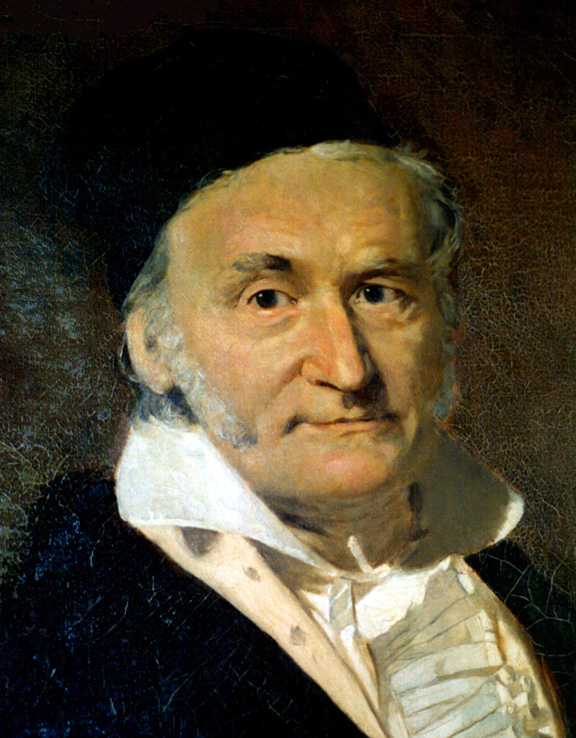
\includegraphics[width= 0.31 \linewidth]{gauss.jpg}
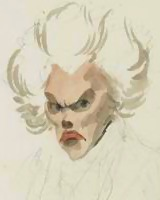
\includegraphics[width= 0.32 \linewidth]{lezhandr.jpg} \end{center} & Метод оценивания параметров эконометрической модели, состоящий в минимизации суммы квадратов расхождений между наблюдаемыми значениями зависимой переменной и значениями этой переменной, вычисленными для наблюдаемых значений независимых переменных по оценённой модели связи.\\
\hline
Обобщённый метод  \newline наименьших квадратов  \newline (GLS) &  \[ (X^T \Omega^{-1} X)^{-1}X^T \Omega^{-1} y\] & \begin{center} 1934 \end{center} & \begin{center}Alexander \\ Aitken \end{center} & \begin{center} не нашёл \end{center} &  Теоретическая процедура оценивания коэффициентов линенйиной модели регрессии в ситуации, когда случайные ошибки имеют разные дисперсии и коррелированы между собой, при этом предполагается, что ковариационная матрица вектора ошибок невырождена и все ее элементы известны. \\
\hline

Взвешенный метод \newline наименьших~квадратов (WLS) & 
\begin{eqnarray*} & (X^T \Omega^{-1} X)^{-1}  X^T \Omega^{-1} y,\\
& \textit{при этом } \\
& \Omega = \diag(\sigma_1,\sigma_2, \ldots \sigma_n) \end{eqnarray*}  &  \begin{center} он же \end{center}& \begin{center}он же \end{center}&\begin{center} не нашел \end{center} & Процедура, состоящая в минимизации определённым образом взвешенной суммы квадратов отклонений наблюдаемых значений зависиммой переменной от значений, вычисляемых по подбираемой модели \newline связи. \\
\hline

Доступный обобщённый \newline метод наименьших \newline квадратов (FGLS) & \[(X^T \hat{\Omega}^{-1} X)^{-1}X^T \hat{\Omega}^{-1} y\] & \begin{center} тот же \end{center} & \begin{center} он же \end{center} & \begin{center} не нашел \end{center} & Практически реализуемая процедура оценивания коэффициентов линейной модели регрессии в ситуации, когда случайные ошибки имеют разные дисперсии и коррелированы между собой, повторяющая процедуру обобщенного метода наисеньших квадратов, но импользующая оцененную ковариационную \newline матрицу вектора ошибок. \\
\hline

Косвенный метод \newline наименьших квадратов \newline (ILS) & & \begin{center} В 1928 начали \newline заниматься \newline проблемой \newline инструментальных переменных \end{center} & \begin{center} Philip Wright \newline Sewall Wright \newline (отец и сын) \end{center} & \center{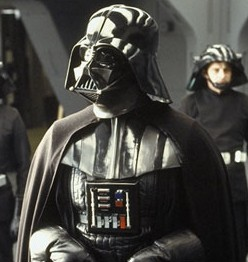
\includegraphics[width=0.4\linewidth]{Darth_Vader.jpg}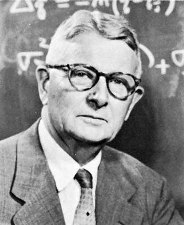
\includegraphics[width= 0.35 \linewidth]{Sewall_Wright.jpg}}  & Mетод получения оценок параметров $i-$го стохастического уравнения структурной формы через оценки наименьших квадратов коэффициентов уравнений приведенной формы. Метод применим в случае точной идентифицируемости $i-$го  структурного \newline уравнения.\\
\hline

Двухшаговый метод \newline наименьших квадратов \newline (2SLS) & \small{\[(X^T Z (Z^T Z)^{-1} Z^T X)^{-1} X^T Z(Z^T Z)^{-1} Z^Ty \]} & \begin{center} 1953 ,  1957 \end{center} & \begin{center} Henri Theil \newline Robert Basmann \end{center} & \begin{center} не нашёл \end{center} &  Метод оценивания коэффициентов уравнения структурной формы, состоящий в предварительной очистке стохастической объясняющей переменой от коррелированности с ошибкой в этом уравнении с использованием инструментальных переменных и в последующем оценивании уравнения, в котором исходная объясняющая переменная заменяется ее очищенным вариантом. \\
\hline
Трёхшаговый метод \newline наименьших квадратов \newline (3SLS) & \[ (\hat Z^T(\hat \Lambda^{-1} \otimes I_g) \hat Z)^{-1} \hat Z^T (\hat \Lambda^{-1} \otimes I_g)y \] &\begin{center} они же \end{center} & \begin{center}они же \end{center} & \begin{center} они же \end{center} & Доступный обобщённый метод наименьших квадратов, применённый к системе одновременных уравнений. Принимает во внимание наличие коррелирванности между ошибками в разных \newline структурных уравнениях. \\
\hline
\end{tabular}}
\end{table}

\end{document}
